%%%%%%%%%%%%%%%%%%%%%%%%%%%%%%%%%%%%%%%%%%%%%%%%%%%
%% P3: Phenomenology of Particle Physics                         
%%
%% Author:  André Rubbia                   		 
%%
%% Figure 2.6 The ratio of the activities as a function of time for different scenarios..
%%
%% This work is licensed under the Creative Commons Attribution 4.0 International License. 
%% To view a copy of this license, visit http://creativecommons.org/licenses/by/4.0/ or 
%% send a letter to Creative Commons, PO Box 1866, Mountain View, CA 94042, USA.
%%
%%%%%%%%%%%%%%%%%%%%%%%%%%%%%%%%%%%%%%%%%%%%%%%%%%%

\documentclass[a4paper,10pt]{article}

\usepackage[T1]{fontenc}
\usepackage[utf8]{inputenc}
\usepackage{lmodern}
\usepackage[labelfont=bf]{caption}
\usepackage{upgreek}
\usepackage{amssymb}
\usepackage{amsmath}

\usepackage{tikz}
\usepackage{pgfplots}
\pgfplotsset{compat=1.17}
\usepgfplotslibrary{ternary}
\usepgfplotslibrary{fillbetween}
\usepgfplotslibrary{external}

\def\d{\mathrm{d}}

\begin{document}

%%%%%%%%%%%%%%%   FIGURE  %%%%%%%%%%%%%%%%%%%%%%%%%%%%%%
\begin{figure}[htb]
\begin{center}
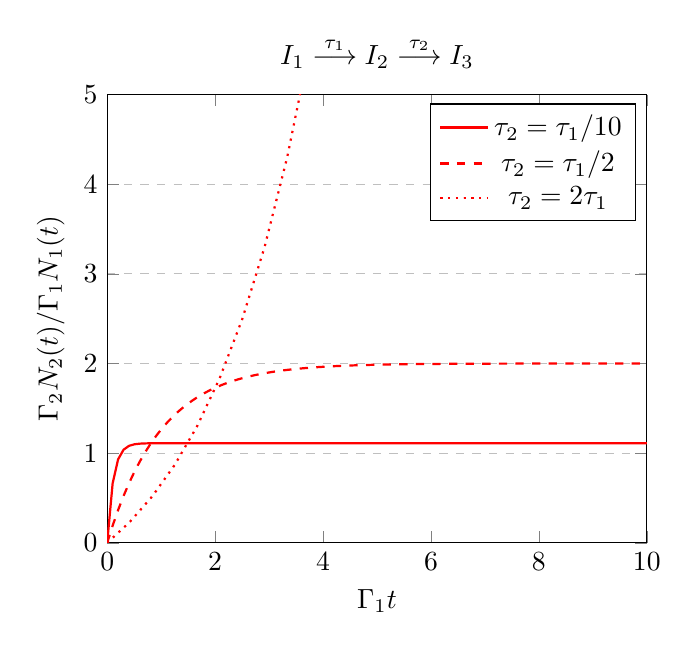
\begin{tikzpicture}[scale=1]
\begin{axis}[
    title={$I_1\overset{\tau_1}{\longrightarrow}
I_2 \overset{\tau_2}{\longrightarrow} I_3$},
    xlabel={$\Gamma_1 t$},
    ylabel={${\Gamma_2 N_2(t)/}{\Gamma_1 N_1(t)}$},
    xmin=0, xmax=10,
    ymin=0, ymax=5,
%    xtick={0,20,40,60,80,100,120,140,160},
%    ytick={1e0,1e1,1e2,1e3,1e4,1e5,1e6,1e7},
%    legend pos=outer north east,
    ymajorgrids=true,
    grid style=dashed,
]
% lambda 2 = 10*lambda_1
 \addplot[domain=0:10,thick, color=red,samples=100] {(10/(10-1))*(1-exp{-(10-1)*x})};
% lambda 2 = 2*lambda_1
 \addplot[domain=0:10,thick, color=red,samples=100,dashed] {(2/(2-1))*(1-exp{-(2-1)*x})};
% lambda 2 = 0.5*lambda_1
 \addplot[domain=0:10,thick, color=red,dotted] {(0.5/(0.5-1))*(1-exp{-(0.5-1)*x})};
     \legend{$\tau_2=\tau_1/10$, $\tau_2=\tau_1/2$, $\tau_2=2\tau_1$}
\end{axis}
\end{tikzpicture}
\caption{The ratio of the activities $\cal R$ of $I_2$ and $I_1$ as a function of time
for different scenarios.}
\end{center}
\end{figure}
%%%%%%%%%%%%%%%   END FIGURE  %%%%%%%%%%%%%%%%%%%%%%%%%%%%%%
%

\end{document}
